% !TEX encoding = UTF-8
% !TEX TS-program = pdflatex
% !TEX root = ../tesi.tex

%**************************************************************
\chapter{Handshake \& Session key}
\label{cap:handshake-session-key}
%**************************************************************

%**************************************************************
\section{How the handshake is structured}

The handshake protocol is used to exchange a session key to encrypt and authenticate all the messages after the handshake. It guarantees perfect forward secrecy and usese nonces both client and server side to deny possible replays attack. The handshake is made of 3 steps that are summarized in the following figure: \ref{fig:handshake}.

\begin{figure}[!h] 
    \centering 
    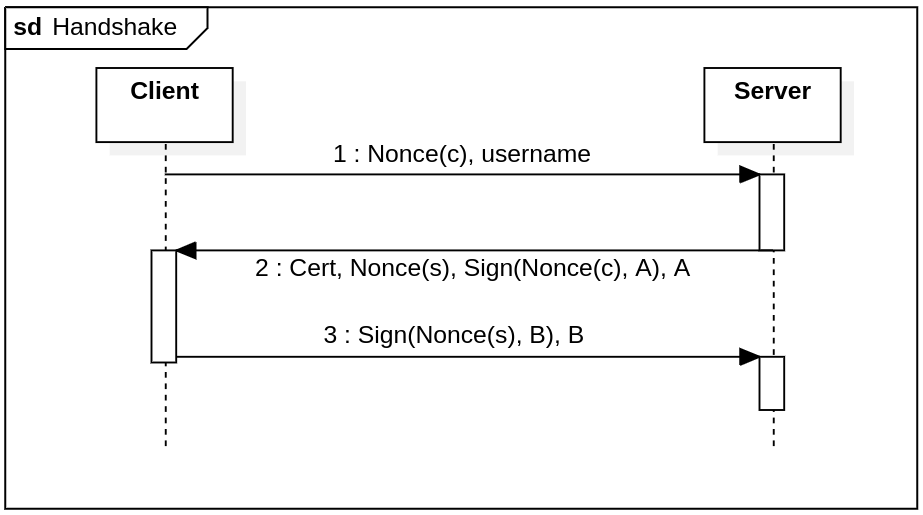
\includegraphics[width=1\columnwidth]{handshake.png} 
    \caption{Handshake.}
    \label{fig:handshake}
\end{figure}

\begin{enumerate}
	\item client sends a random number also called nonce and the chosen username;
	\item server checks validity of username and prepares the preliminary steps to generate a shared session key:
	\begin{itemize}
		\item checks if the username does not contain invalid characters, only alphanumeric and dot characters (.) strictly not in the first position are allowed. If the username is not valid connection is closed allerting the client;
		\item checks if the username is registered, if not then the connection gets closed by sending an error message to the client;
		\item choses a random number \(\alpha\) and uses it to calculate the public Diffie-Hellman key that we will call ``A'' as A = \(g^\alpha mod p \);
		\item the server now sends his certificate, a random number and ``A''. It also signs, using the server private RSA key, the random number received from the client Nonce(c) and A together and sends the signature to the client.
	\end{itemize}
	\item the client checks validity of certificate and signature and generates the shared session key:
	\begin{itemize}
		\item validates server certificate using the CA;
		\item uses server public key to validate the signature received;
		\item choses a random number \(\beta\) and uses it to calculate the public Diffie-Hellman key that we will call ``B'' as B = \(g^\beta mod p \);
		\item generates shared secret Kab = \(g^{\alpha*B} mod p\);
		\item generates shared key hashing Kab with SHA256 and truncating the result to 128 bits;
		\item signs, using the client private RSA key, the random received Nonce(s) and ``B'';
		\item eliminates ``A'', ``B'', \(\alpha\);
		\item sends the generated signature. 
	\end{itemize}
	\item the server checks validity of signature and generates the shared session key:
	\begin{itemize}
		\item uses client public key to validate the signature received;
		\item generates shared secret Kab = \(g^{\beta*A} mod p\);
		\item generates shared key hashing Kab with SHA256 and truncating the result to 128 bits;
		\item eliminates ``A'', ``B'', \(\beta\);
	\end{itemize}	 
\end{enumerate}

%**************************************************************
\section{How is the session key used}

%**************************************************************